% Standalone manuscript results spread. Place article-comparison.pdf beside this file.
\documentclass[sigconf,anonymous,nonacm]{acmart}
\settopmatter{printacmref=false,printccs=false,printfolios=false}
\setcopyright{none}
\hypersetup{bookmarks=false,pdfsubject={Matched full-article modeling experiments}}
\title{Which Analyses Survive a Change in the Virtual Pairing?}
\author{Anonymous Author(s)}
\begin{document}
\begin{teaserfigure}
  \centering
  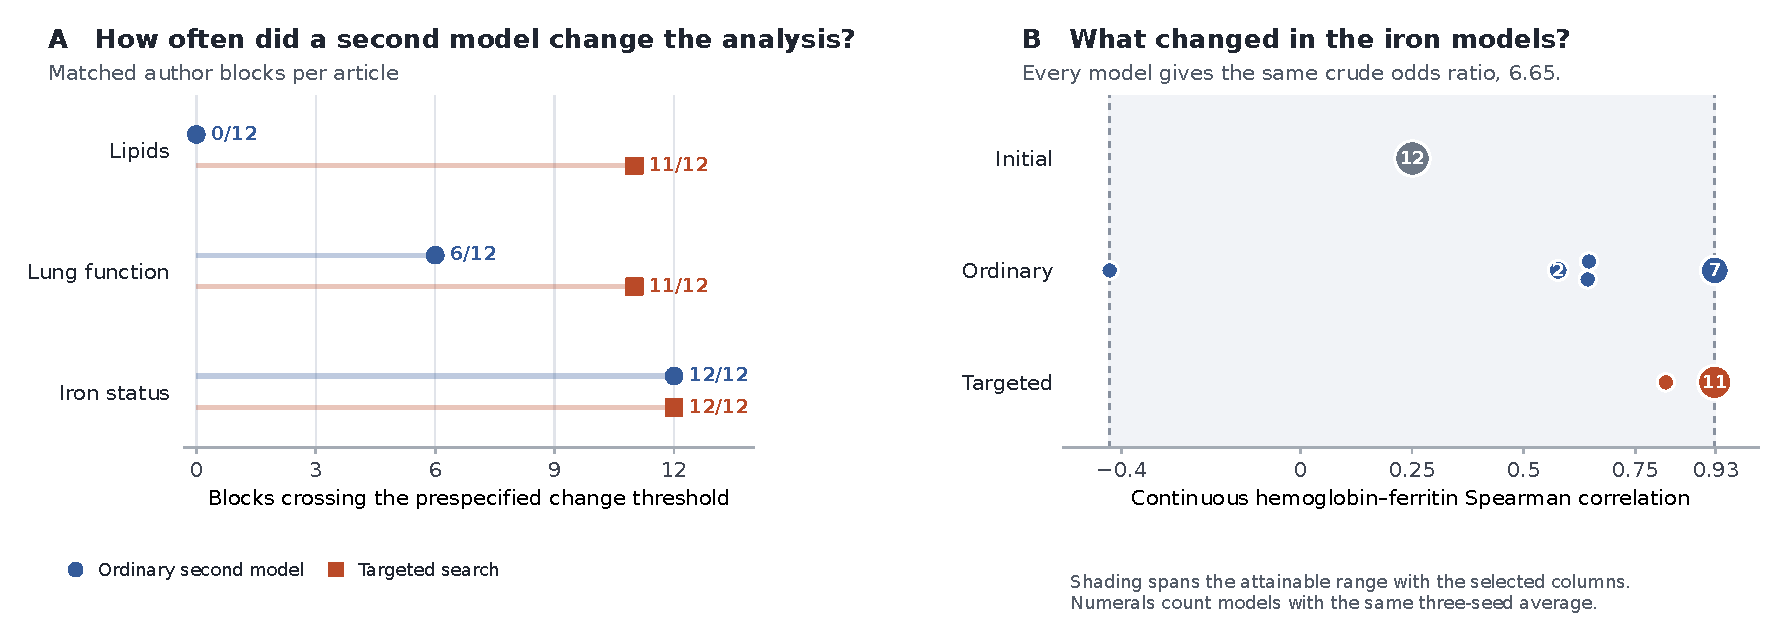
\includegraphics[width=.97\textwidth]{article-comparison.pdf}
  \caption{Two follow-ups shared the source article and the initial program. Panel A counts blocks in which another admissible program materially changed the requested analysis. Panel B places the iron programs inside the exact feasible bounds for the selected marginal columns and hemoglobin bands. Panel B's bound was calculated after scoring.}
  \Description{Of twelve blocks per article, ordinary and targeted requests changed lipid screening in zero and eleven, lung screening in six and eleven, and iron correlation in twelve and twelve. With the iron odds ratio fixed, correlations span minus 0.427 to 0.928.}
\end{teaserfigure}
\maketitle
\raggedbottom
\pagestyle{empty}
\thispagestyle{empty}

\section*{From an article to a scientific use}
How many adults would meet a non-HDL cholesterol screening threshold of 160~mg/dL? A Tanzanian study reports total and HDL cholesterol summaries. Subtracting the two means fixes mean non-HDL. To count individuals above the cutoff, a researcher also needs to know which total and HDL measurements belong to the same person. A scientific agent can make that assignment explicit in code and generate a second cohort to test its consequences.

\paragraph{Matched authoring.}
Twelve initial GPT sessions per paper read its original scientific text, extracted the relevant statistics, and wrote a sampler. We supplied the marginal grid conventions and scientific estimators. Two follow-ups independently received the same first program. One requested another defensible model. The other also asked for an alternative within-person pairing that materially changed the intended analysis, in either direction. The agent chose and implemented the pairing. A program had to pass the source checks at all three seeds. The outcome counted changes exceeding the prespecified pooled and seed-level margins. All twelve assigned blocks per paper entered the denominator.

\paragraph{A change of use exposes the assumption.}
Across lipid models, mean non-HDL stayed at 128.77~mg/dL. Ordinary and targeted follow-ups changed the screening estimate by a median of 0.27 and 13.18 percentage points. On Polish lung volumes, a sex-specific regression and correlation still permitted different fractions below an individual FEV1/FVC of 0.70. Ordinary and targeted median changes were 7.31 and 24.76 points among eleven eligible pairs. Five discordant blocks favored targeted search (two-sided paired \(p=0.0625\)). A post-hoc check found a median 15.28\% of targeted records within 0.005 of the cutoff, versus 2.63\% for ordinary models. This qualifies how a clinician should read these constructed scenarios.

\paragraph{Where an ordinary second model suffices.}
The Chinese iron study supplies four counts that fix the crude anemia odds ratio at 6.65. All 36 programs recovered it. Continuous hemoglobin--ferritin rank correlation, however, changed materially in all 12 blocks under \emph{both} follow-ups. Seven blocks even produced byte-identical ordinary and targeted assignments. The selected columns admit correlations of \(-0.427\) and \(0.928\) by reversing or preserving ferritin rank within each hemoglobin band. All twelve initial authors returned the same seeded assignments. Independent authorship can therefore give unanimous answers where the science admits opposite signs.

\paragraph{Scope of the evidence.}
The three experiments cover 36 assigned author blocks, 106 calls and 315 independently recalculated virtual tables. Their contribution is an executable test of whether a scientific answer changes under a documented modeling choice. Estimating agreement in people requires a measured comparator. For example, in a separate prospective grip analysis a frozen model predicted a 3.81~kg average absolute between-hand gap, compared with 3.30 and 3.78~kg in the two primary measured samples. Those results answer a different, complementary question.
\end{document}
